\section{Experimental evaluation}
\label{sec:research-questions-and-scenario}
One of the research questions behind the experiment was to test the style model and the plasticity model of the companion proposed. 

In this experiment, the same styles - Authoritative and Permissive -  as the ones were applied to the robots were used.
From these previous results, Authoritative and Permissive styles seemed to be identifiable by parents and applicable to the Nao robot \cite{Johal2014}. 

With this experiment, we wanted to verify our plasticity framework applied to HRI in a more general manner. 
In that sense, this experiment was also questioning versatile vs specialist robots. 
The aim here was to collect opinions of parents and children on the versatility of a companion robot and see if it was preferable to have a companion robot able to play several roles or does it affect its credibility and trust in accomplishing the tasks to be versatile.

In the experiment scenario, the child alone at home has to review his multiplication tables. 
His Teacher companion is here to ask him questions and to check if he knows them. 
After some questions, the companion(s) propose to dance for the child (faking that it has a dance competition) taking the Buddy role. 
However, some more questions of the math quiz have to be answered by the child and the companion retakes the Teacher role.


Following are a list of our principal hypothesis :
\begin{itemize}[noitemsep,nolistsep]
	\item[H0] Authoritative robots are perceived to be more dominant than permissive by children.
	\item[H1] Styles influence children's attitude in an interactive task.
	\item[H2] Styles influence the perceived competence and credibility of the robot in an interactive task.
	\item[H3] Styles influence the complicity with the robot in an interactive task.
	%\item[H4] Versatility of a companion increases the attachment and engagement of the children in interaction with it.
	\item[H4] Role-Specialist robots are perceived to be more competent and trustworthy than versatile robots.
	%\item[H6] There is an influence of the style during the math quiz during the dance on the child's behaviour.
\end{itemize}
%todo sentence for expe Within subjects with put the conditions
\subsection{Subjects/Participants}
16 children and their relatives participated to the experiment. 
Most often, the relatives were parents, but 3 children came with their grand-parents.
16 children participated to the experiment with ages from 7 to 11 y.o (M:\dots, SD \dots).
There was \dots girls and \dots boys. 
%todo boy and girl, and age and sd of age

\subsection{Apparatus/Materials}
The experiment took place in an ecological environment in the Domus apartment (see Fig. ~\ref{fig:domusroof}).
\footnote{Domus is an experimental platform of the LIG Laboratory of Grenoble-Alps in France, fully equipped and functional apartment with a kitchen, an office/living-room (where the experiment took place) and  a bedroom (where the interviews of the children took place)
	A sound and video direction room, from where the parents and another experimenter accessed audio and video capture in the apartment and record from the control PCs}
We added a Kinect sensor in order to record data. 
The Domus apartment is controllable by the OpenHab\footnote{\url{http://www.openhab.org}} middle-ware. 
OpenHab is a home control middle-ware that supports various sensors, protocols and operating systems. 
We were able, for instance, to launch music on the speaker of the apartment directly form the robot, by doing a simple HTTP\_REQUEST. 
\begin{figure}[h]
	\begin{tabular}{c c}
		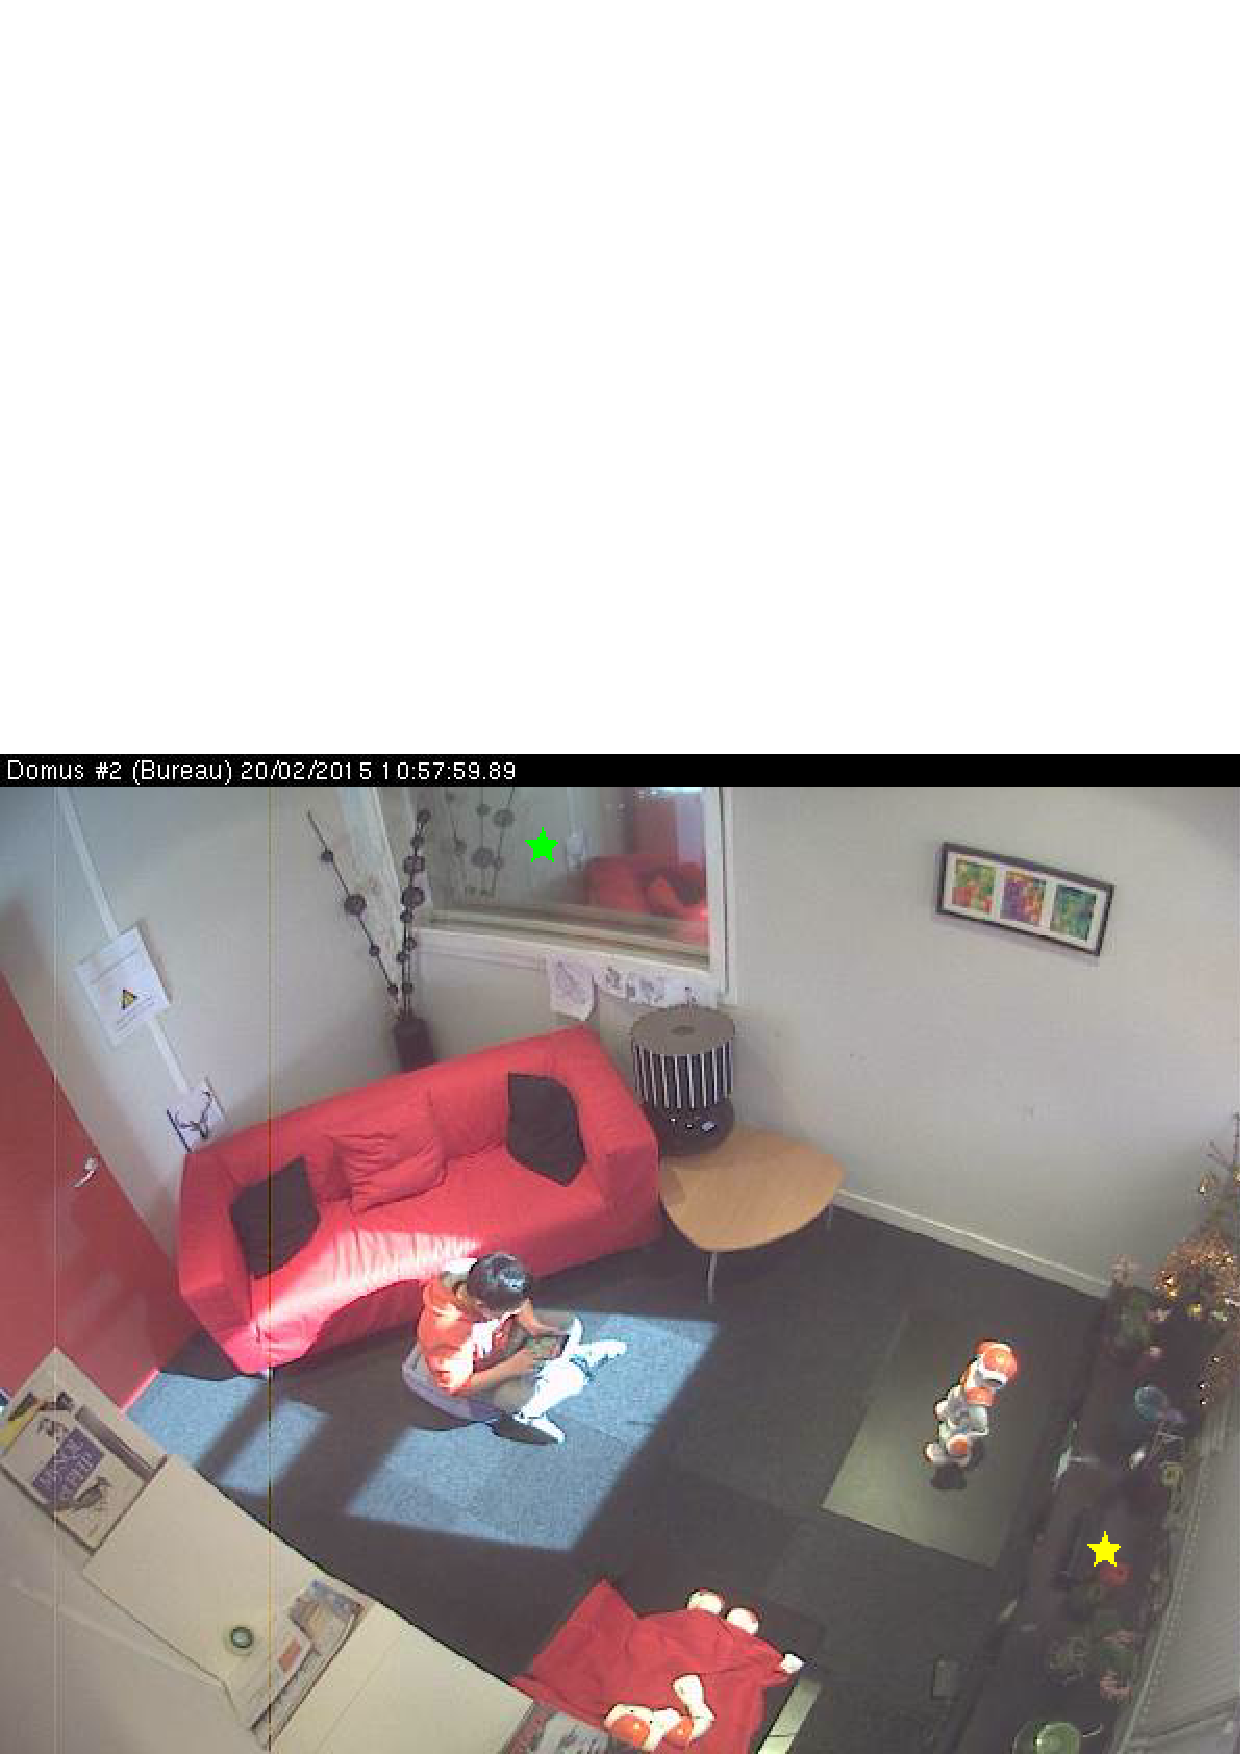
\includegraphics[width=0.45\linewidth]{Figures/illustrate/roof1}&
		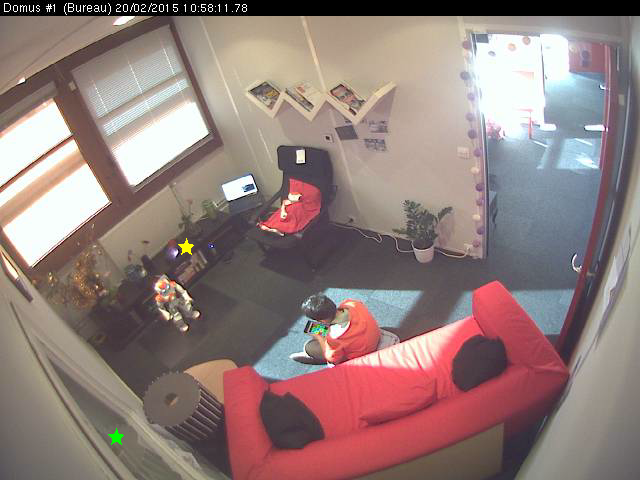
\includegraphics[width=0.45\linewidth]{Figures/illustrate/roof2}
	\end{tabular}
	\caption{Experimental Settings}
	\label{fig:domusroof}
\end{figure}
Each interaction with the Nao robot(s) lasted about 15 minutes. 
Every child passed two sessions in a counterbalanced manner. 
For every child, we had about 30 minutes of recording of the interaction itself (a bit more because we also recorded explanations of the experimentalist). 
 
